% Q19: source PDF p3; one tile and its four rotated copies.
% Coordinates are schematic and introduce no numerical labels.
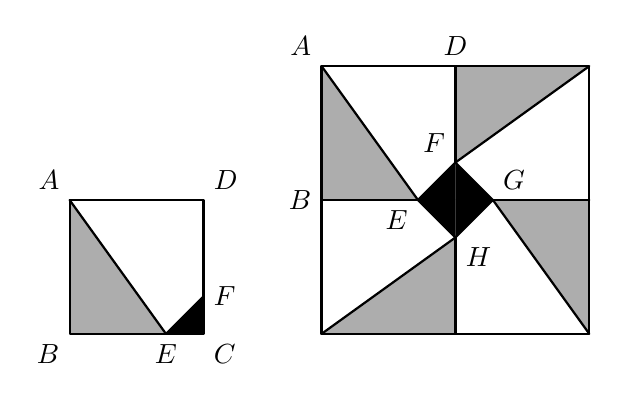
\begin{tikzpicture}[line cap=round,line join=round,thick]
\begin{scope}[scale=1.7]
  \fill[black!32] (0,1)--(0,0)--(.72,0)--cycle;
  \fill[black] (1,0)--(1,.28)--(.72,0)--cycle;
  \draw (0,0) rectangle (1,1); \draw (0,1)--(.72,0)--(1,.28);
  \node[above left] at (0,1) {$A$}; \node[below left] at (0,0) {$B$};
  \node[below right] at (1,0) {$C$}; \node[above right] at (1,1) {$D$};
  \node[below] at (.72,0) {$E$}; \node[right] at (1,.28) {$F$};
\end{scope}
\begin{scope}[xshift=3.2cm,scale=1.7]
  \foreach \angle in {0,90,180,270}{
    \begin{scope}[shift={(1,1)},rotate=\angle,shift={(-1,-1)}]
      \fill[black!32] (0,2)--(0,1)--(.72,1)--cycle;
      \fill[black] (1,1)--(1,1.28)--(.72,1)--cycle;
      \draw (0,2)--(.72,1)--(1,1.28);
    \end{scope}
  }
  \draw (0,0) rectangle (2,2);
  \draw (0,1)--(.72,1) (1.28,1)--(2,1) (1,0)--(1,.72) (1,1.28)--(1,2);
  \node[above left] at (0,2) {$A$}; \node[left] at (0,1) {$B$};
  \node[above] at (1,2) {$D$};
  \node[below left] at (.72,1) {$E$}; \node[above left] at (1,1.28) {$F$};
  \node[above right] at (1.28,1) {$G$}; \node[below right] at (1,.72) {$H$};
\end{scope}
\end{tikzpicture}
